The derivation of fragility models requires the definition of a criterion to allocate one (or multiple) structures into a set of damage states, according to their nonlinear structural response. These rules to relate structural response with physical damage can vary significantly across the literature. Displacement-based methodologies frequently adopt the strain of the concrete and steel (e.g. \cite{BorziEtAl2008b}; \cite{SilvaEtAl2013}). The vast majority of the methodologies that require equivalent linearisation methods or nonlinear time history analysis adopt inter-storey drifts (e.g. \cite{VamvatsikosCornell2005}; \cite{RossettoElnashai2005}), or spectral displacement calculated based on a pushover curve (e.g. \cite{Erberik2008}; \cite{SilvaEtAl2014c}). The various rules dictated by the damage model are currently being stored in a \verb=csv= file (tabular format), as described below for each type of model. Tabel \ref{table:dmg_list} reports the available damage models and for each of them the methodologies in which they can be used.

\begin {table}[!htbp]
\caption{List of damage models and methodologies in which they can be used}
\label{table:dmg_list}
\begin{center}
  \begin{tabular}{|l|l|}\hline
\textbf{Type} & \textbf{Methodologies} \\ \hline
Strain dependent & D-BELA capacity curves generation\\ 
							& SP-BELA capacity curves generation\\ \hline
Capacity curve dependent &  Record-based nonlinear static procedure\\ 
										& Nonlinear Time History Analysis on SDOF\\ \hline
Spectral displacement &  Record-based nonlinear static procedure\\ 
										& Nonlinear Time History Analysis on SDOF\\ \hline
Interstorey drift & Record-based nonlinear static procedure\\ 
						& Nonlinear Time History Analysis on SDOF\\
						& Direct nonlinear static procedures\\ \hline
  \end{tabular}
\end{center}
\end{table}

\subsubsection{Strain-based damage criterion}
\label{subsubsec:strain-dmg}
Displacement-based \citep{CrowleyEtAl2004} or mechanics-based \citep{BorziEtAl2008b} methodologies use strain levels to define a number of limit states. Thus, for each limit state, a strain for the conrete and steel should be provided. It is recognized that there is a large uncertainty in the allocation of a structure into a physical damage state based on its structural response. Thus, the Risk Modeller's Toolkit allows the representation of the damage criterion in a probabilistic manner. This way, the parameter that establishes the damage threshold can be defined by a mean, a coefficient of variation and a probabilistic distribution (normal, lognormal or gamma) \citep{SilvaEtAl2013}. This approach is commonly used to at least assess the spectral displacement at the yielding point (\verb=Sdy=) and for the ultimate capacity (\verb=Sdu=). Other limit states can also be defined using other strain levels (e.g. \cite{CrowleyEtAl2004}), or a fraction of the yielding or ultimate displacement. For example, \cite{BorziEtAl2008b} defined light damage and collapse through the concrete and steel strains, and significant damage as $^3/_4$ of the ultimate displacement (\verb=Sdu=).\\

To use this damage criteria, it is necessary to define the parameter \verb=Type= as \verb=strain dependent= within the damage model file. Then, each limit state needs to be defined by a name (e.g. light damage), type of criterion and the adopted probabilistic model. Using the damage criteria described above (by \cite{BorziEtAl2008b}), an example of a damage model is provided in Table~\ref{table:strain-dmg}. In this case, the threshold for light damage is defined at the yielding point, which in return is calculated based on the yielding strain of the steel. The limit state for collapse is computed based on the mean strain in the concrete and steel (0.0075 and 0.0225, respectively) and the a coefficient of variation (0.3 and 0.45, respectively). The remaining limit state (significant damage), is defined as fraction (0.75) of the ultimate displacement (collapse).

\begin {table}[!htbp]
\caption{Example of a strain dependent damage model}
\label{table:strain-dmg}
\begin{center}
  \begin{tabular}{ | c | c | c | c | c |}
  \hline
Type & strain dependent &  &  &  \\ \hline
Damage States & Criteria & distribution & mean & cov  \\ \hline
light damage & Sdy & lognormal &  & 0 \\ \hline
significant damage & fraction Sdu & lognormal & 0.75 & 0 \\ \hline
collapse & strain & lognormal & 0.0075 0.0225 & 0.30 0.45 \\ \hline
  \end{tabular}
\end{center}
\end{table}

\subsubsection{Capacity curve-based damage criterion}
\label{subsubsec:cc-dmg}
Several existing studies (e.g. \cite{Erberik2008}; \cite{SilvaEtAl2014c}; \cite{CasottoEtAl2005}) have used capacity curves (spectral displacement versus spectral acceleration) or pushover curves (roof displacement versus base shear) to define a set of damage thresholds. In the vast majority of these studies, the various limit states are defined as a function of the displacement at the yielding point (\verb=Sdy=), the maximum spectral acceleration (or base shear), and / or of the ultimate displacement capacity (\verb=Sdu=). For this reason, the mechanism that has been implemented in the RMTK is considerably flexible, and allows users to define a set of limit states following the options below:\\

\begin{enumerate}
 \item \verb=fraction Sdy=: this limit state is defined as a fraction of the displacement at the yielding point (\verb=Sdy=) (e.g. 0.75 of \verb=Sdy=)
 \item \verb=Sdy= this limit state is equal to the displacement at the yielding point, usually marking the initiation of structural damage.
 \item \verb=max Sa= this limit state is defined at the displacement at the maximum spectral acceleration.
 \item \verb=mean Sdy Sdu= this limit state is equal to the mean between the displacement at the yielding point (\verb=Sdy=) and ultimate displacement capacity (\verb=Sdu=).
 \item \verb=X Sdy Y Sdu= this limit state is defined as the weighted mean between the displacement at the yielding point (\verb=Sdy=) and ultimate displacement capacity (\verb=Sdu=). X represents the weight associated with the former displacement, and Y corresponds to the weight of the latter (e.g. 1 Sdy 4 Sdu).
 \item \verb=fraction Sdu= this limit state is defined as a fraction of the ultimate displacement capacity (\verb=Sdu=) (e.g. 0.75 of \verb=Sdy=)
 \item \verb=Sdu= this limit state is equal to ultimate displacement capacity (\verb=Sdu=), usually marking the point beyond which structural collapse is assumed to occur.\\
\end{enumerate}

In order to create a damage model based on this criterion, it is necessary to define the parameter \verb=Type= as \verb=capacity curve dependent=. Then, each limit state needs to be defined by a name (e.g. slight damage), type of criterion (as defined in the aforementioned list) and a potential probabilistic model (as described in the previous subsection). An example of a damage model considering all of the possible options described in the previous list is presented in Table~\ref{table:cc-dmg}, and illustrated in Figure~\ref{fig:cc-dmg}. Despite the inclusion of all of the options, a damage model using this approach may use only a few of these criteria. Moreover, some of the options (namely the first, fifth and sixth) may by used multiple times.

\begin {table}[!htbp]
\caption{Example of a capacity curve dependent damage model.}
\label{table:cc-dmg}
\begin{center}
  \begin{tabular}{ | c | c | c | c | c |}
  \hline
    Type & capacity curve dependent &  &  & \\ \hline
    Damage States & Criteria & distribution & Mean & Cov \\ \hline
    LS1 & fraction Sdy & lognormal & 0.75 & 0.0 \\ \hline
    LS2 & Sdy & normal &  & 0.0 \\ \hline
    LS3 & max Sda & normal &  & 0.0 \\ \hline
    LS4 & mean Sdy Sdu & normal &  & 0.0 \\ \hline
    LS5 & 1 Sdy 2 Sdu & normal &  & 0.0 \\ \hline
    LS6 & fraction Sdu & normal & 0.85 & 0.0 \\ \hline
    LS7 & Sdu & normal &  & 0.0 \\ \hline
  \end{tabular}
\end{center}
\end{table}

\begin{figure}[htb]
  \centering
      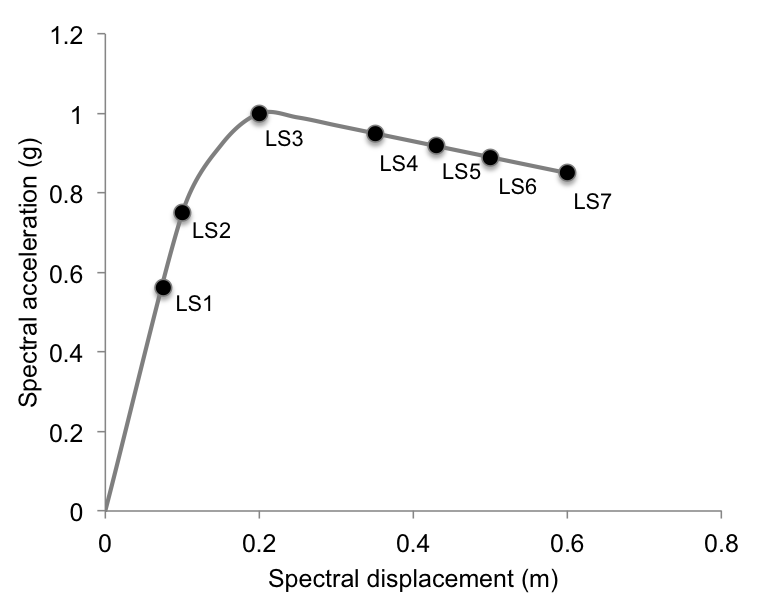
\includegraphics[width=9cm]{figures/cc_damage_model.png}
  \caption{Representation of the possible options for the definition of the limit states using a capacity curve.}
  \label{fig:cc-dmg}
\end{figure}

\subsubsection{Spectral displacement-based damage criterion}
\label{subsubsec:sd-dmg}
In many methodologies for the definition of the seismic vulnerability of structures an equivalent Single Degree Of Freedom (SDOF) system is subjected to multiple analyses instead of the complex Multi Degree Of Freedom (MDOF) system. The capacity of the structure is thus expressed in terms of spectral acceleration vs spectral displacement. The easiest way to allocate the structure into a damage state is that of comparing spectral displacement demand with spectral displacement damage thresholds. A damage model has been implemented in the RMTK that allows to introduce directly spectral displacement damage thresholds, and an example of input file is provided in Table~\ref{table:sd-dmg}. A single value of mean and coefficient of variation for each damage threshold should specified for the entire building class.

\begin {table}[htb]
\caption{Example of a spectral displacement based damage model}
\label{table:sd-dmg}
\begin{center}
  \begin{tabular}{ | c | c | c | c | c | c |}
  \hline
    Type & spectral displacement &  & \\ \hline
    Damage States & distribution & Mean & Cov \\ \hline
    Slight & lognormal & 0.01 & 0.0 \\ \hline
    Moderate & lognormal & 0.05  & 0.1 \\ \hline
    Exyensive & lognormal & 0.1  & 0.2 \\ \hline
    Collapse & lognormal & 0.2  & 0.25 \\ \hline
  \end{tabular}
\end{center}
\end{table}

\subsubsection{Inter-storey drift-based damage criterion}
\label{subsubsec:isd-dmg}
Maximum inter-storey drift is recognised by many researchers (e.g. \cite{VamvatsikosCornell2005}; \cite{RossettoElnashai2005}) as a good proxy of the damage level of a structure, because it can detect the storey by storey state of deformation as opposed to global displacement.

The use of this damage model is quite simple: the parameter \verb=Type= in the csv file should be set to \verb=interstorey drift= and inter-storey drift thresholds need to be defined for each damage state, in terms of median value and dispersion.

The probabilistic distribution of the damage thresholds implemented so far is lognormal. A different set of thresholds can be assigned to each structure, as in the example provided in Table~\ref{table:isd-dmg}, but also a single set can be defined for the entire building population to be assessed.

When a vulnerability assessment methodology uses an equivalent SDOF system instead of the complex MDOF system it is still possible to define an inter-storey drift-based damage model for the MDOF system and introduce a relationship to convert inter-storey drift to spectral displacement damage thresholds. The conversion file containing the relationship between the maximum inter-storey drift along the building height and the spectral displacement of the equivalent SDOF system can be obtained using the "Conversion from MDOF to SDOF" module (see Section \ref{sec:mdof_to_sdof}). If this option wants to be enabled the variable \verb=deformed shape path= should be set to \verb=TRUE= in the csv input file, and the name of the conversion file should be specified in the next cell, as shown in Table ~\ref{table:isd-dmg}. The conversion file should be placed in the same folder where the damage model is located. An example of conversion file is provided in Table ~\ref{table:isd-sd} for the vulnerability assessment of a building population. In the conversion file the User has the option of specifying either a single conversion relationship for the entire building class or one for each capacity curve of the building class.

\begin {table}[htb]
\caption{Example of a inter-storey drift based damage model}
\label{table:isd-dmg}
\begin{center}
  \begin{tabular}{ | c | c | c | c | c | c |}
  \hline
    Type & interstorey drift &  &  & & \\ \hline
    deformed shape path & TRUE & ISD-Sd.csv  &  & & \\ \hline
    Damage States & distribution & Median & Dispersion & Median & Dispersion \\ \hline
    LS1 & lognormal & 0.001 & 0.0 & 0.001 & 0.0 \\ \hline
    LS2 & lognormal & 0.01  & 0.2 & 0.015 & 0.0 \\ \hline
    LS3 & lognormal & 0.02  & 0.2 & 0.032 & 0.0 \\ \hline
  \end{tabular}
\end{center}
\end{table}

\begin {table}[htb]
\caption{Example of file containing the relationship between maximum inter-storey drift and spectral displacement for each structure of the building population}
\label{table:isd-sd}
\begin{center}
  \begin{tabular}{ | c | c | c | c | c | c |}
  \hline
    ISD & 0.0004 & 0.0009 & 0.0013 &	0.0018 & 0.0023 \\ \hline
    Sd [m] & 0.003 &	0.006 & 0.009 &	0.012 &	0.015 \\ \hline
    ISD & 0.0003 & 0.0011 & 0.0014 &	0.002 & 0.0025 \\ \hline
    Sd [m] & 0.002 &	0.005 & 0.011 &	0.013 &	0.014 \\ \hline
    ISD & ... & ... & ... &	... & ... \\ \hline
    Sd [m] & .. &... & ... &... &... \\ \hline
  \end{tabular}
\end{center}
\end{table}